%!TEX root = artem_kotov_v1.tex
\section{Task 4}

\begin{task}
    Определить, какая из величин $a, b, d$ вносит наибольший вклад в уточнение прогноза для величины c (в смысле дисперсии распределения).
\end{task}


Проведенный численный эксперимент показал, что для первой модели условия $\D [c|d] < \D [c|b]$ и $\D [c|d] < \D [c|a]$ выполняются для любых допустимых значений $a \in [75, 90]$, $b \in [500, 600]$ и $d \in [0, 1380]$. Однако для второй модели это оказывается неверным, к сожалению, аналитически показать это строго пока не удалось, т.е. может быть так, что это просто численная ошибка, но я, скорее, склоняюсь к тому, что это свойства модели.

\begin{figure}[H]
    \centering
    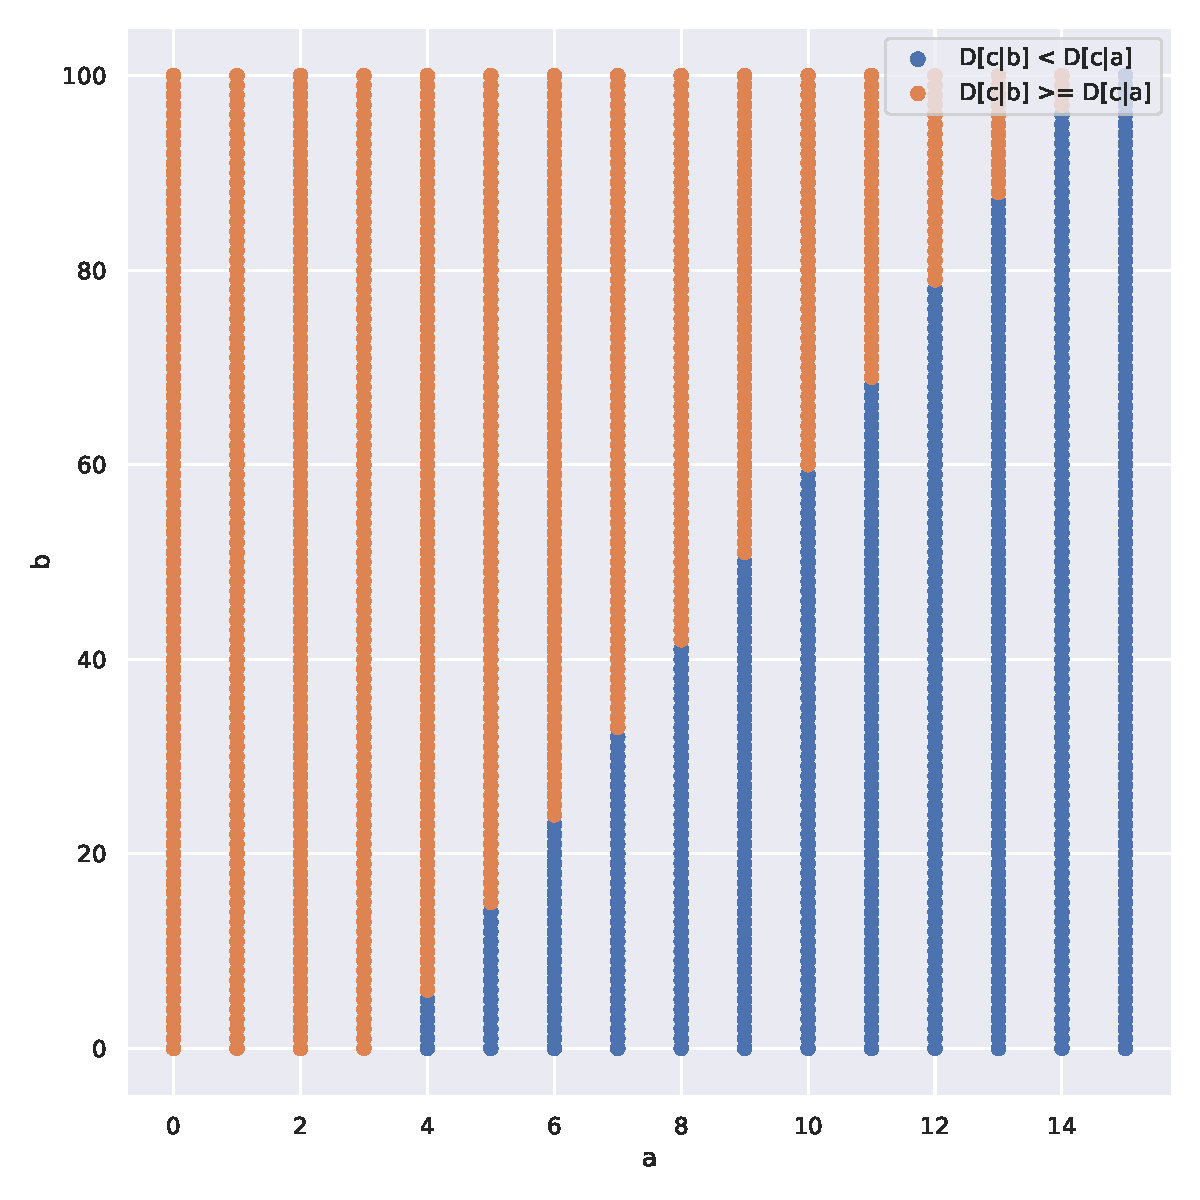
\includegraphics[width=0.7\textwidth]{pics/task4_1.pdf}
    \caption{График множества точек ${(a, b): \D [c|b] < D[c|a]}$ (синий) и ${(a, b): \D [c|b] \ge D[c|a]}$ (оранжевый) для первой модели.}
\end{figure}

\begin{figure}[H]
    \centering
    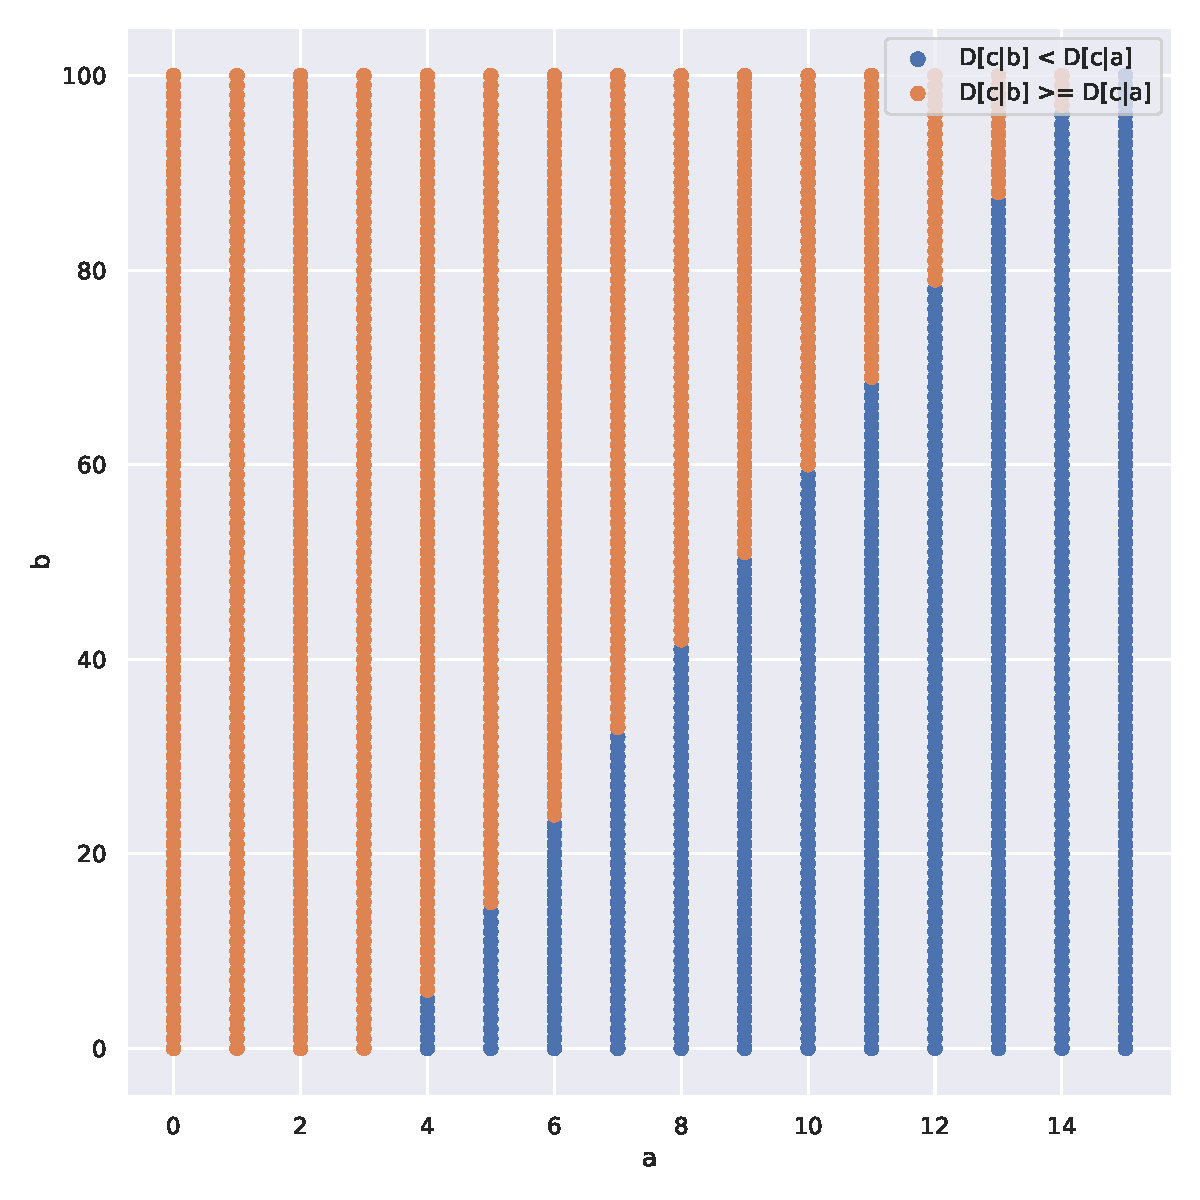
\includegraphics[width=0.7\textwidth]{pics/task4_1.pdf}
    \caption{График множества точек $\{(a, b): \D [c|b] < D[c|a]\}$ (синий) и $\{(a, b): \D [c|b] \ge D[c|a]\}$ (оранжевый) для второй модели.}
\end{figure}

В целом, из графиков можно сделать вывод, что эти множества таки линейно разделимы для обоих моделей.
